\documentclass[letterpaper, 10 pt, conference]{ieeeconf}  
\IEEEoverridecommandlockouts
\usepackage{enumerate}
\usepackage{graphicx}
\usepackage{amsmath}
\usepackage[english]{babel}
\usepackage{blindtext}

\title{On New Collision Detection Techniques: Minkowski Sums, Fourier Transforms and Spherical Decomposition}
\author{Can Erdogan \\ CS6491: Computer Graphics \\ Final Project \\ 2015-12-01}

\begin{document}
\maketitle

% -------------------------------------------------------------------------------------------------
% -------------------------------------------------------------------------------------------------
\begin{abstract}

Collision detection is a vital tool for robotics, computer graphics and mechanical design.
However, in most of the literature, the analysis of collision detection is performed only in cartesian
space although recent work, Lysenko's 2013 paper \cite{lysenko2013fourier}
and Behandish's 2016 paper \cite{behandish2016analytic}, propose a paradigm shift into frequency
domain. In this report, we being with the background information on Minkowski sums, spherical
decompositions and Fourier transforms, to analyze the main advantages that
underlie these papers. We conclude that the gist of the papers lie within the power of FFTs in computing Minkowski sums, and the advantage of 
spherical decompositions over uniform samples (along with NFFTs), and provide preliminary
results from our own implementations that confirm the findings of the authors.
\end{abstract}


% -------------------------------------------------------------------------------------------------
% -------------------------------------------------------------------------------------------------
\section{Introduction}

Collision detect is one of the fundamental tools for robotics, computer graphics and mechanical 
design. A number of different variants of collision detection is investigated within these fields
with examples ranging from static and dynamic objects in the environment to narrowphase and 
broadphase (single vs. multiple collisions) detections. In this work, we are interested in
the collision of a single pair of static objects. The body of the work is focused on examining
the role of three concepts: (1) Minkowski sums, (2) fourier transformations and (3)
spherical decompositions.

It is a well-known fact that Minkowski sums can be utilized to generate more complex shapes
from simpler primitives. One of the main observations that motivate our research is the utilization
of Fourier transforms to increase the efficiency of their computations. A second motivation is to
observe the effect of shape representation in the efficiency of Fourier transforms and the exploitation
of their underlying properties such as the \textit{convolution theorem} and the \textit{time shifting}.
The bulk of the work is focused on the recent work (2016) of Behandish and Ilie \cite{behandish2016analytic}
who promote the use of spherical decompositions along with non-equispaced Fast Fourier transforms (NFFTs).

\begin{figure}[ht!] 
  \centering
  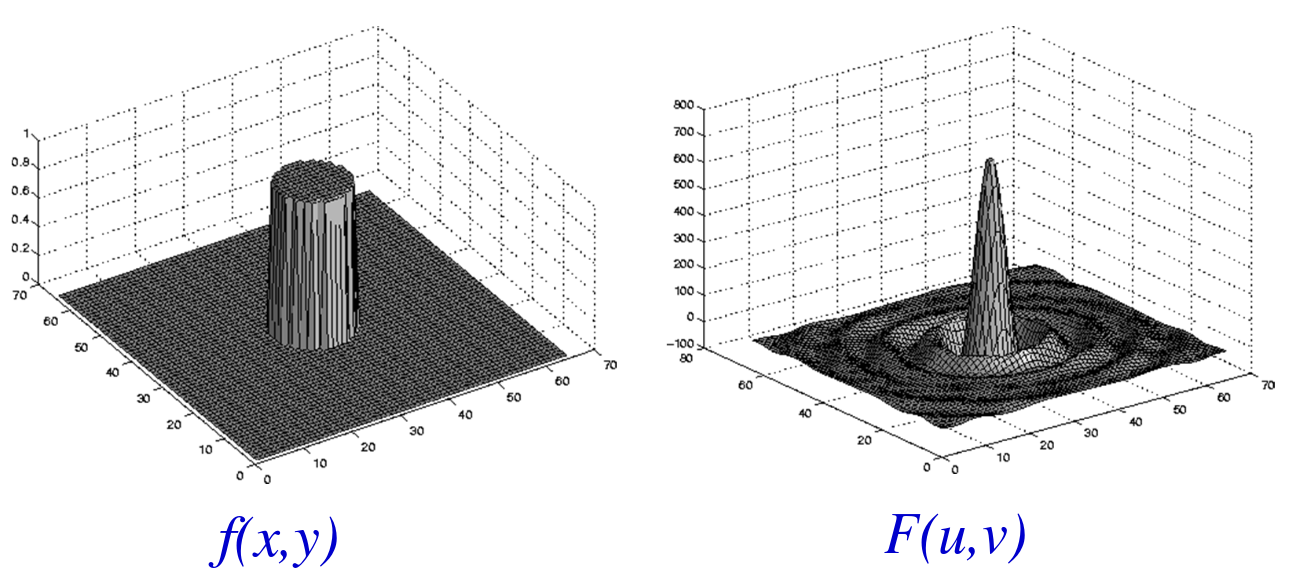
\includegraphics[width=1.0\linewidth]{Figures/main.png}
  \caption{An obstacle in the cartesian space and its representation in the frequency domain}
  \label{fig:main}
\end{figure}

Figure \ref{fig:main} represents one of the key ideas that allow the transformation of object representations
in cartesian space to the frequency space. The idea is that some function $f(x,y)$ (in $\mathbf{R}^2$ for
this example) can be used to represent a cylindrical object (possible an obstacle) and if this so-called
\textit{bump function} is chosen properly (e.g. smoothness, differentiability, etc.), its Fourier transform,
$F(x,y)$, can be exploited in collision detection computations.

This report is organized as follows. First, we present briefly the related work in Fourier transforms,
their use for collision detection in robotics, and the variants of shape descriptors in computer graphics.
Then, we present the idea of Minkowski sums and bump functions to formulate collision detection
rules. In Section IV, we briefly give an overview of the idea of spherical decomposition and its use 
with bump functions, followed by in Section V, with the main treatment of Fourier transformations in
the context of collision detection. We conclusion with preliminary results that confirm the 
findings of \cite{behandish2016analytic} and point out to a number of future speed-up techniques
accumulated from different sources (\cite{behandish2016analytic, kavraki1995computation, lysenko2013fourier}).

% -------------------------------------------------------------------------------------------------
% -------------------------------------------------------------------------------------------------
\section{Related Work}

The Fourier transform, reportedly first used by Carl Friedrich Gauss to compute the period of
an asteroid as a series of sinusoids, has been the linchpin of modern signal processing techniques
since the introduction of Fast Fourier Transforms (FFT)s in 1965 \cite{cooley1965algorithm}. There 
are two key properties that are of interest of FFTs to our work. First, the FFT algorithm computes
the Fourier transform of a discrete signal of length $n$ in O(nlogn) time whereas the classical 
discrete transformation by definition takes O($n^2$) computations. Second, the Fourier transform
of a function in cartesian space represents the data in terms of a summation of different
frequencies. As in \cite{lysenko2013fourier}, we propose the use of this representation by 
first analyzing the values at the higher frequencies and stop the computation of the transformation
if the lack of a collision can be guaranteed. 

One of the key ideas of this work is how the shape representation affects the collision detection
methods. A number of shape descriptors have been proposed in the computer graphics literature 
such as the OBB trees \cite{gottschalk1996obbtree} and voxel-based representations \cite{sagardia2014new}.
The benefit of spherical decompositions is that every sub-part is rotation-invariant and although
within the scope of this work, we limit ourselves to spheres of constant radius, the extension
to variable radii is trivial \cite{behandish2016analytic}. 

The use of spherical decompositions leads to an interesting area of fourier computations,
namely nonequispaced Fast Fourier transforms (FFTs). The traditional DFT algorithm and the
FFT algorithm both assume that the time-varying signal is sampled with equispaced time 
intervals. Although this might be the case with a lot of traditional electrical sensors,
a number of domains such as health sector (MRIs) \cite{knopp2007note}, computational
physics (heat flow computations) \cite{lee2005type}, etc. have sampled from non-equispaced
time nodes. In our domain, the placement of the sphere centers are clearly non-uniform
and \cite{behandish2016analytic} proposed the use of NFFT algorithms to compute
the Fourier transform of a signal composed of their locations. We have examined a number
of prior work in this field \cite{dutt1993fast, dutt1995fast, potts2001fast} and foresee
that the use of these algorithms will increase the efficiency of the Fourier approach
even more \cite{keiner2009using}. However, within the scope of this work, we limit
ourselves to interpolating between the centers of the spheres and generating a 
sparse uniform signal. 

% -------------------------------------------------------------------------------------------------
% -------------------------------------------------------------------------------------------------
\section{Minkowski Sums in Collision Detection}

\subsection{Bump functions}

The two main shape representations we discuss in this work is uniform-sampling and
spherical-sampling which can be interpreted as a list of voxels with 0-1 booleans
for where the voxel intersects the shape and a number of 3D points where spheres
of some constant radii are within the shape. In discussing such representations,
our papers of interest \cite{behandish2016analytic, lysenko2013fourier} choose the adopt 
the descriptor functions $f_S: \mathbf{R}^3 \rightarrow \mathbf{R}$ for
some solid $S$ such that the shape is the domain of $f_S$ where $f_S(x) > 0$. 
This representation is convenient because if we formalize the idea above with
the notation:

\begin{equation}
 U_t(f_S) = \{x \in \text{domain of} \; f_S | f_S(x) > t\},
\end{equation}

then, the union and the intersect of two shapes $S_1$ and $S_2$ become additions and 
dot product of their respective descriptor functions:

\begin{align}
 S_1 \cup S_2 &= U_0(f_{S_1} + f_{S_2}) \\
 S_1 \cap S_2 &= U_0(f_{S_1}f_{S_2})
\end{align}

For instance,
in classical robotics applications, with voxel-based descriptors, the function
$f_S = \mathbf{1}_S$ is an indicator function such that $\mathbf{1}_S(x) = 1$
if and only if $x \in S$. In such a case, two shapes can only intersect if there
exists some $x$ such that both of the shapes have some volume, that is
both $f_{S_1}(x) = f_{S_2}(x) = 1$ and thus, their dot product is greater than 0.
Note that since the analytical expressions of shape descriptors is too complex,
when we refer to operations on these functions, we imply to operations on a set of sampled
values in their domains. 

A number of different variants of descriptor functions are available in addition
to indicator functions that have more smoothness properties and in this work,
for the spherical decomposition approach, we are interested in the following
bump function:

\begin{equation}
 \psi_\alpha(x) = 
 \begin{cases}
    e^{{(1-|x|^{-\alpha}})^{-1}},& \text{if } |x| < 1\\
    0,              & \text{otherwise}
\end{cases}
\end{equation}

\noindent which is parameterized by constant $\alpha$ that changes how
the function behaves close to the non-zero limits. For a single sphere shape $S_0$,
we then define the descriptor function as $f_{B_0} = \psi_\alpha(|x|/r)$ where
$r$ is the radius of the shape. In Figure \ref{fig:bumpAlphas}, we demonstrate
the effect of the $\alpha$ value in the descriptor function outputs. In our 
work, we adopted $\alpha = 1$. Note that $\alpha = \infty$ corresponds to the
indicator function $\mathbf{1}_S(x)$. 

\begin{figure}[ht!] 
  \centering
  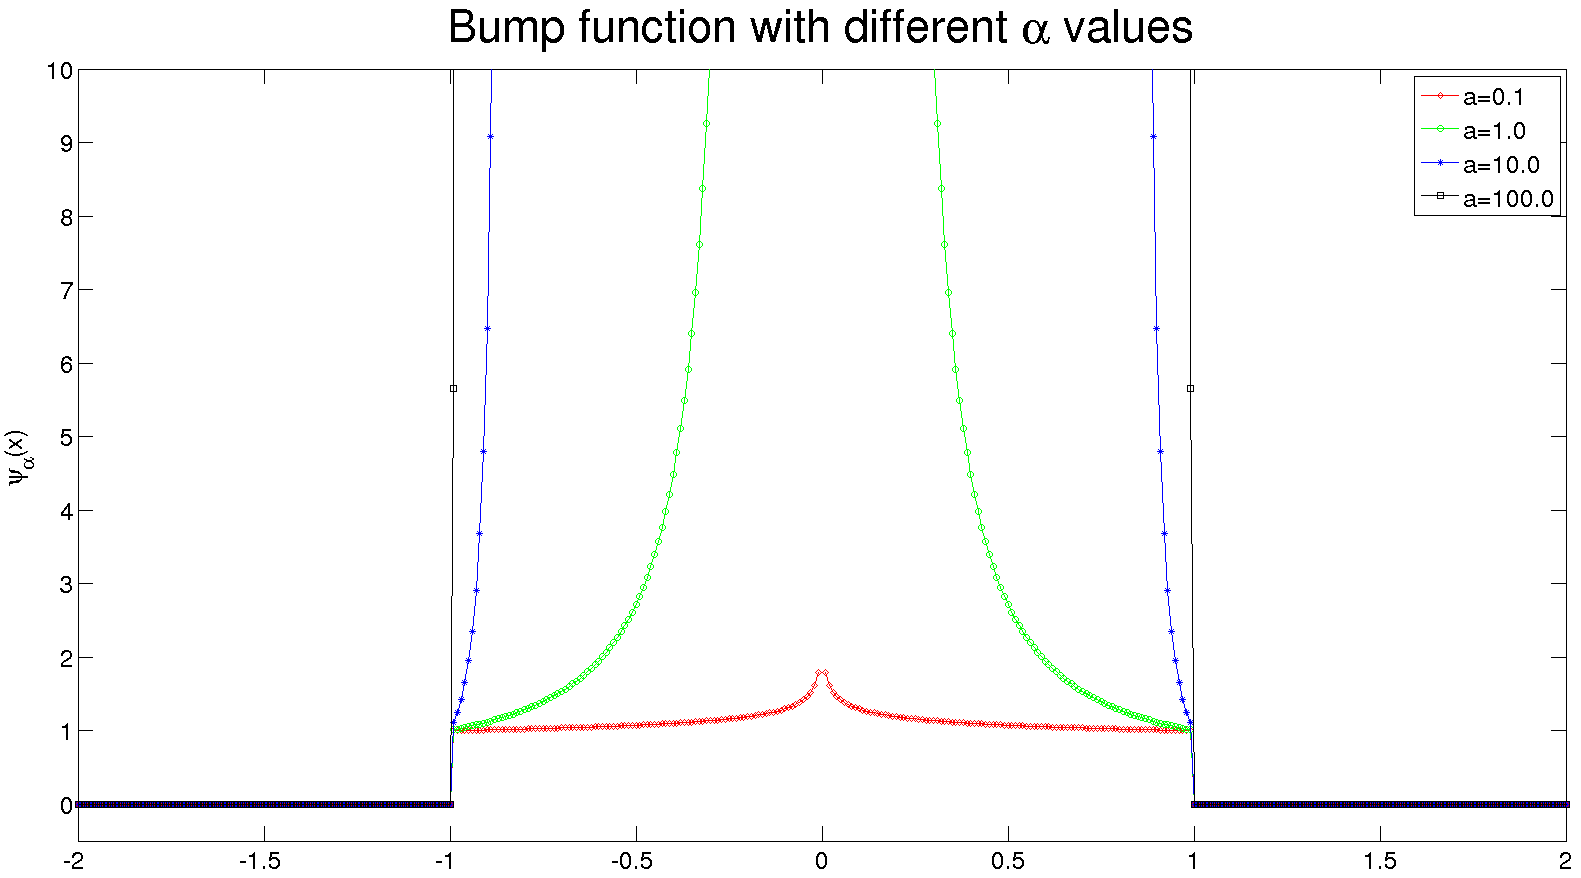
\includegraphics[width=1.0\linewidth]{Figures/bump.png}
  \caption{The effect of the $\alpha$ constants in the descriptor function.}
  \label{fig:bumpAlphas}
\end{figure}

\subsection{Use of Minkowski Sums in Early-Miss Tests}


\begin{figure*}[ht!] 
  \centering
  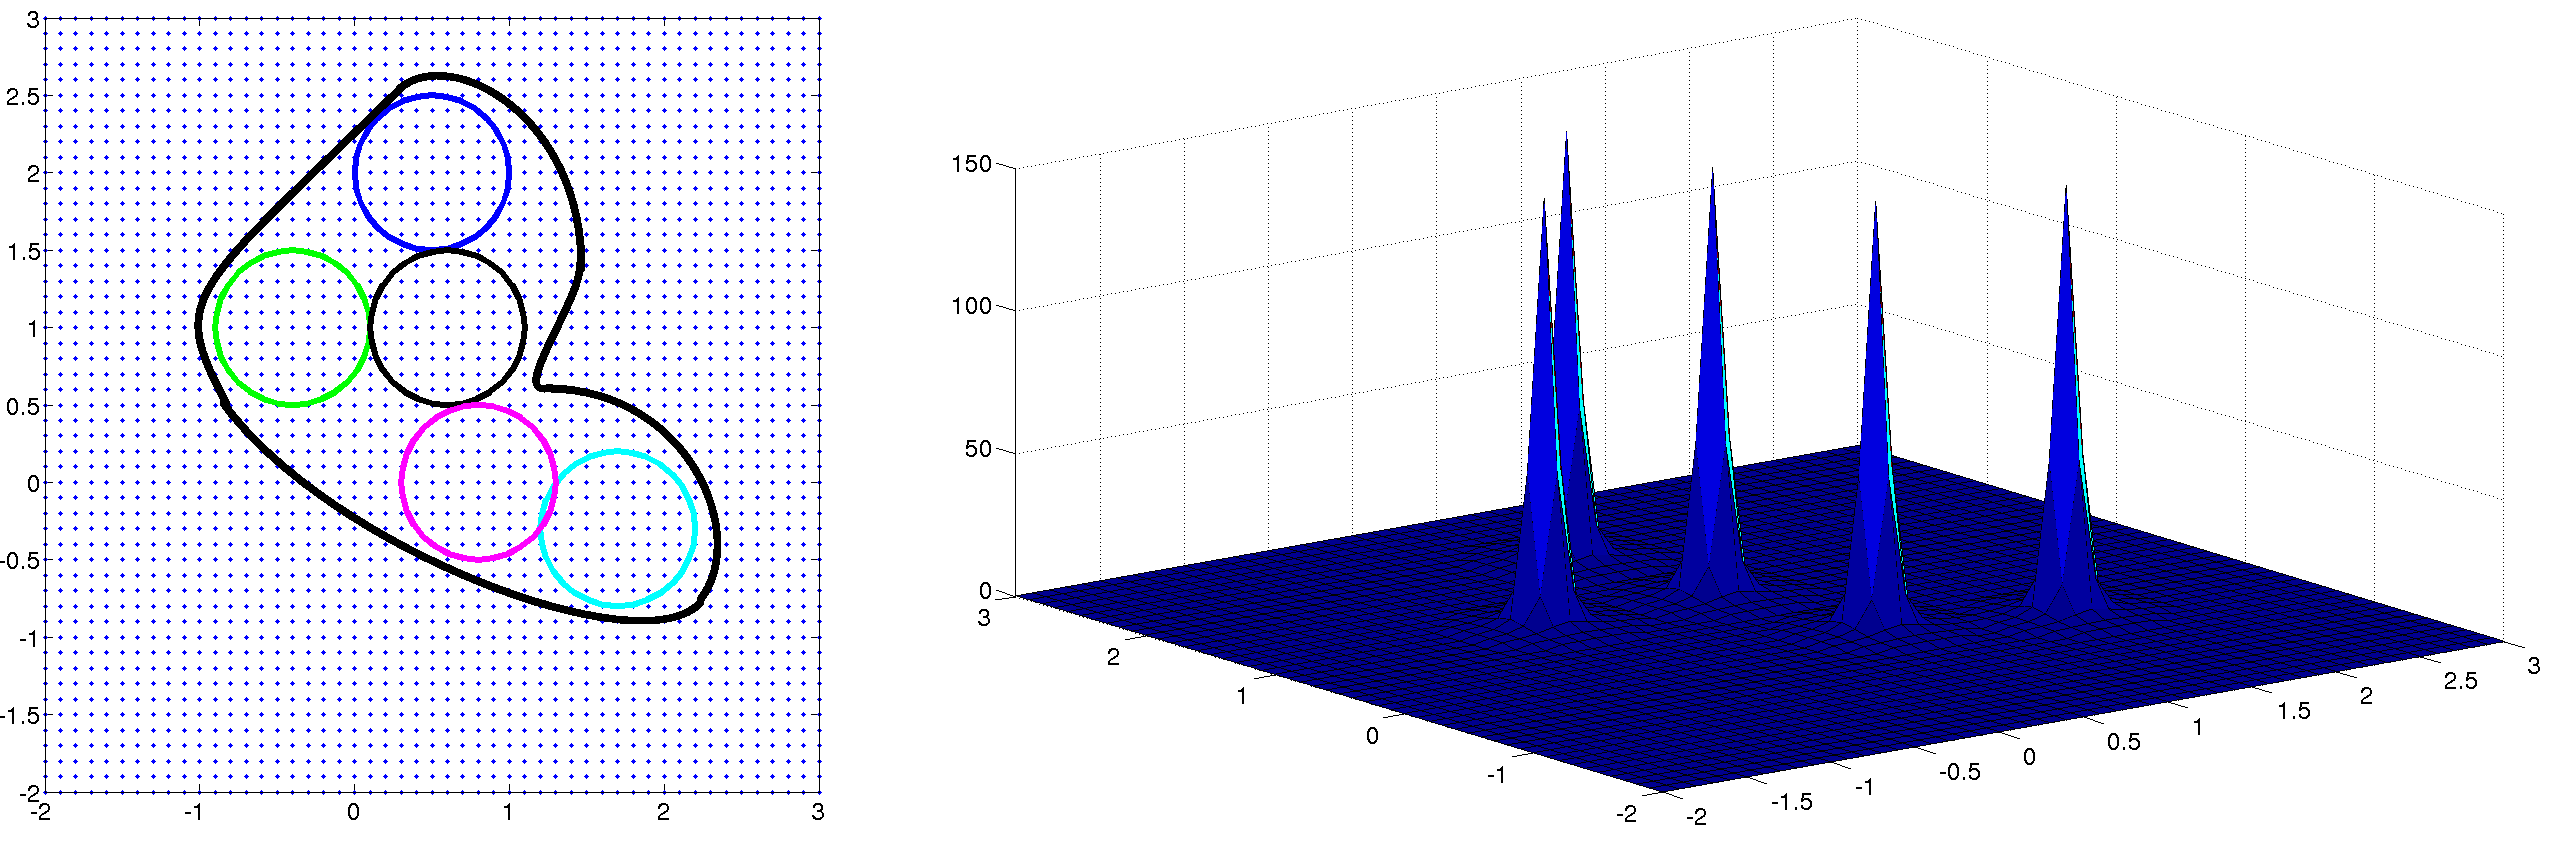
\includegraphics[width=1.0\linewidth]{Figures/bumpConvolved.png}
  \caption{An example of spherical decomposition for a 2D shape and the visualization of the
  shape descriptor function composed of the individual bump functions of the spheres.}
  \label{fig:bumpConvolved}
\end{figure*}

An important observation made in \cite{lysenko2013fourier} is that in most applications, 
the frequency of non-collisions is much higher than collisions. Thus, it is important to bias
our computations towards detecting lack of collisions early on with so-called ``early-miss'' tests.
One example of such early-miss tests is the common adopted of bounding boxes in computer graphics,
specifically ray tracing applications. 

Here, we make a brief note on how the Minkowski sum, can be utilized to implement such a early-miss test. 
First, a brief definition: for two sets $A$ and $B$, their Minkowski sum $A \oplus B$ is defined as
the set:

\begin{equation}
 A \oplus B = \{a+b | a \in A, b \in B\}
\end{equation}

\noindent where, in some applications, it is insisted that for one of the sets, say $A$, the origin $O \in A$. 

The idea behind using the Minkowski sum is to swell up one of the objects say, $S_2$ with a third object
$M$ such that, the negative result of the test $S_1 \cap (S_2 \cup M)$ implies that $S_1 \cap S_2 = \emptyset$.
Clearly, for some choices of $M$, such as elliptic objects, this early-miss test is more efficient. 
Note that the shape descriptor of the Minkowski sum of two objects $M$ and $N$ can be expressed as a convolution of their shape descriptors, a property
that will be useful in the frequency space analysis:

\begin{equation}
M \cup N = U_0(f_M \ast f_N)  
\end{equation}

\noindent where the $\ast$ represents the convolution of the two functions. To learn more about the 
Fourier interpretation of this operation, see the section ``Convolution theorem'' in Section V.
Note that the early-miss test $S_1 \cap (S_2 \cup M)$ now contains two integrals, one for
the convolution and one for the dot product, and in Section V, we will discuss how this situation
can be remedied with Fourier transforms.

% -------------------------------------------------------------------------------------------------
% -------------------------------------------------------------------------------------------------
\section{Spherical Decomposition}

Spherical decomposition of three-dimensional objects has been well studied in the computer graphics
literature. One of the classical approach is based on the medial axis transform (MAT) where the idea
is to represent the shape using spheres with maximal radius such that they are tangential to the
inner surface of the object manifold. A challenge with medial axis approaches is that the MAT of 
an r-set is not necessarily closed, a property that is desirable and achievable with the Minkowski
sum formulation we will show in the next section. Instead, \cite{behandish2016analytic} proposes
a variant of the sphere packing algorithms that exploit the signed distance function field representation
of an object, with reportedly less number of output spheres.

In the left image of Figure \ref{fig:bumpConvolved}, we demonstrate a spherical decomposition of a
two-dimensional object. The idea is to accumulate the bump functions of each sphere, to approximate
the overal shape descriptor function as shown on the right. Next, we formulate this approach using
Minkowski sums that will help us exploit Fourier representation in Section V.

\subsection{Minkowski Sum Formulation}

Let $P$ be the set of center points of the balls $B_i$ that are used to describe an object shape
$S \approx \hat{S} = \bigcup B_i$. The idea is that the approximate shape $\hat{S}$ can be described
as a Minkowski sum of a base ball $B_0$ and the set of center points $P$. Here, we explain 
the proof in \cite{behandish2016analytic} to justify this expansion. We begin with the 
basic description of union of objects as defined in Equation 2:

\begin{equation}
 f_{\hat{S}}(x) = \sum_i f_{B_i}(x) = \sum_{p_i \in P} f_{B_0}(x - p_i)
\end{equation}

\noindent where the use of the central ball $B_0$ is justified by the offset $(x-p_i)$. Then, we 
expand the definition of the ball description function as:

\begin{equation}
 f_{\hat{S}}(x) = \sum_i \int_{\mathbf{R}^3} \delta^3(x^\prime-p_i)[f_{B_0}(x-x^\prime) dx^\prime
\end{equation}

\noindent which allows us to reason about the centers of the balls $p_i$ in the continuous samples
$x^\prime$. This is significant because in the next step, by defining a function of spatial impulses,

\begin{equation}
 \rho(x) := \sum_i \delta^3(x-p_i)
\end{equation}

\noindent, where $\delta^3$ is a Dirac function, we can now rewrite the
Minkowski sum of the approximate shape $\hat{S}$ as a convolution of the
primitive ball function $B_0$ and the points:

\begin{equation}
 P \oplus B_0 = U_0(\rho \ast f_{B_0})
\end{equation}

This result is encouraging because first, we have already seen the use of Minkowski sums in early-miss
tests and we hope to exploit frequency domain properties in their computations. Second, Lysenko provides
theoretical bounds on the Hausdorff distances for Minkowski sum approximations which can be transferred
to spherical decomposition approximations. \cite{lysenko2013fourier}

% -------------------------------------------------------------------------------------------------
% -------------------------------------------------------------------------------------------------
\section{Fourier transforms}

\begin{figure*}[ht!] 
  \centering
  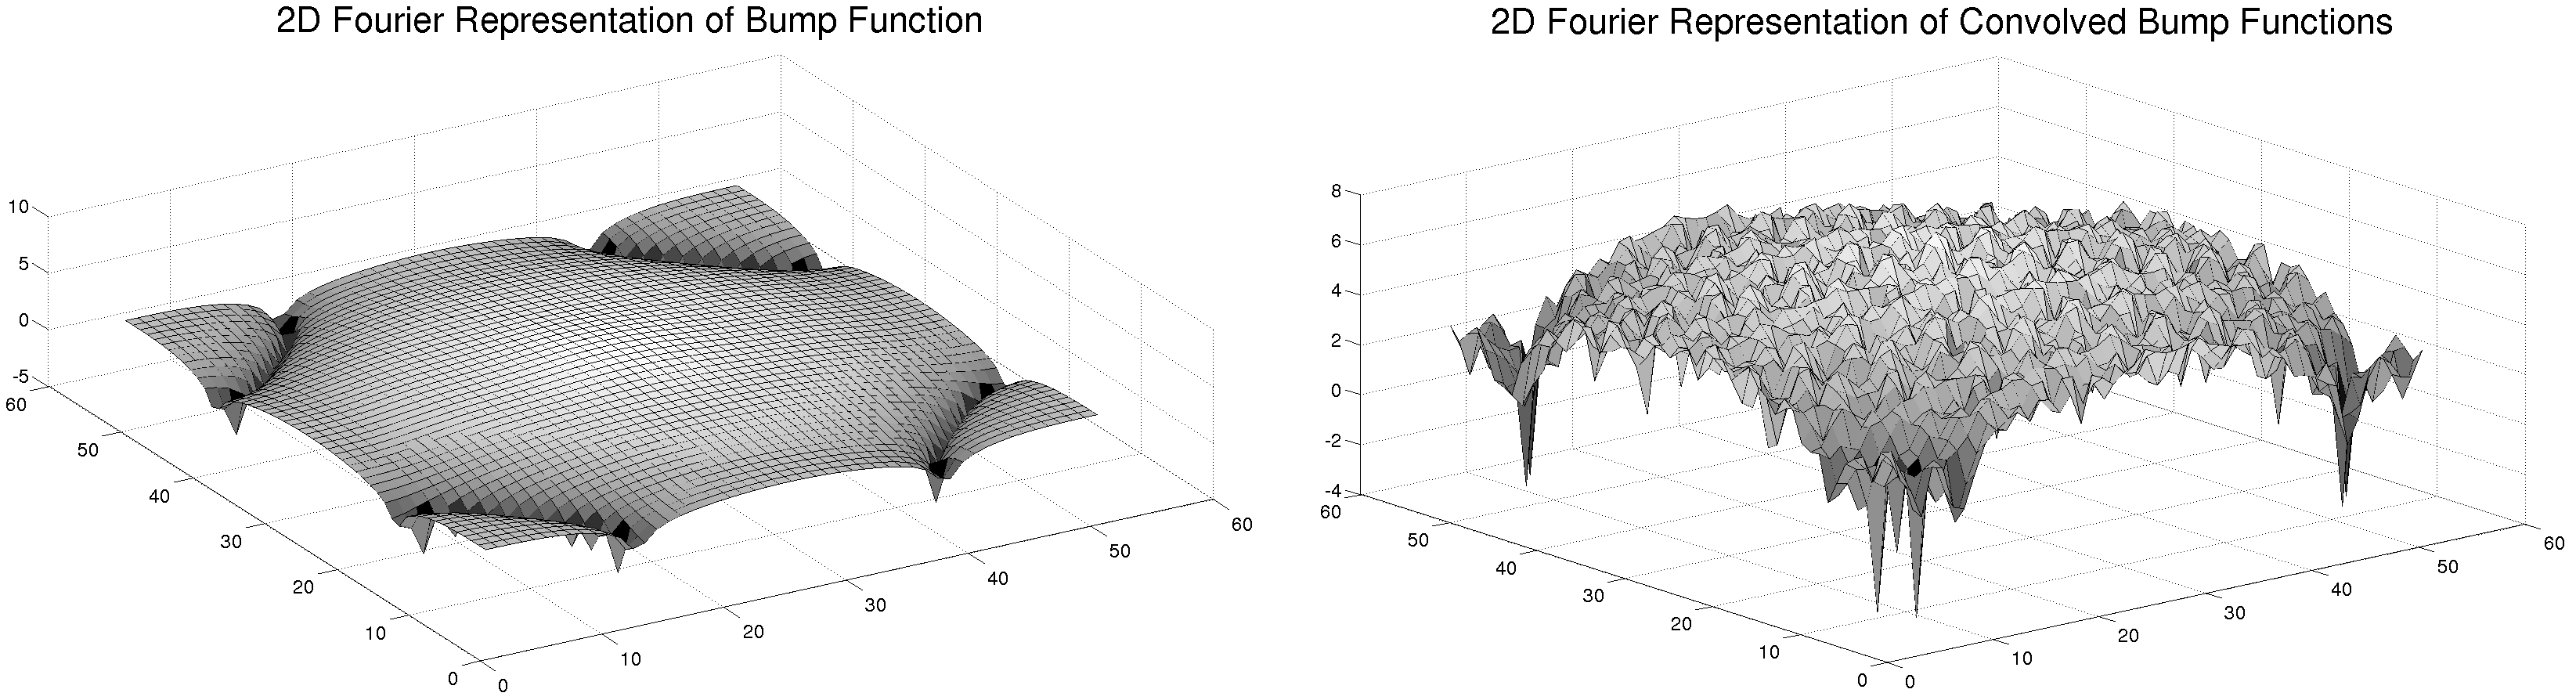
\includegraphics[width=1.0\linewidth]{Figures/bumpFouriers.png}
  \caption{The frequency domain representations of the $B_0$ function and the descriptor function for the shape in Figure 3.}
  \label{fig:bump}
\end{figure*}

\subsection{Convolution theorem}

For two functions $f_1$ and $f_2$ and their corresponding Fourier transforms $F_1$ and $F_2$, the
following two identities hold true under suitable conditions:

\begin{align}
 F(f_1 \ast f_2) &= F_1 \cdot F_2 \\ 
 F(f_1 \cdot f_2) &= F_1 \ast F_2
\end{align}

\noindent where $\cdot$ represents a point-wise multiplication and the function $F(.)$ takes the Fourier transform
of its input. This indicates that the convolution steps for the Minkowski sums of the descriptor functions
can be implemented as point-wise multiplications. This is indeed very powerful because the Minkowski sum 
is an $O(n^2)$ operations whereas the Fourier transform is $O(n)$ and the FFT algorithm is $O(nlog(n))$. 

Figure 4 demonstrates, on the left, the Fourier domain representation of the bump function defined in Equation 4 implemented
for 2D objects. On the right, we observe the Fourier representation of the entire shape description function
for the shape in Figure 3, generated by the convolution of the bump functions in the frequency space. 

One advantage of using the spherical decomposition also comes out in the Fourier representation where we can precompute
the transform of the function $B_0$ to any desired resolution and then convolve it with the list of ball centers
online. Note that to match the signal lengths, the center list would need to be padded with zeros as FFT is applied. 

\subsection{Cartesian Transformations with Dirac functions}

Kavraki's initial work on Fourier domain representations of configuration spaces in 1995 \cite{kavraki1995computation} 
dealed only with translations of obstacles and the robot agents. To the most part, most of the literature still focuses
mostly on translations, and has heuristic approaches for approximating rotations. Although it should be noted that
it is trivial to reflect rotations of multiples of $\tfrac{pi}{4}$ in the frequency domain. The advantage for
the translations is based on the fact that they can be represented as time-shifts where for some signal
$f(x)$, the Fourier transform of its shift by $\Delta x$, $f(x - \Delta x)$ is:

\begin{equation}
 f(x - \Delta x) = e^{-2\pi i \Delta x} F(x)
\end{equation}

\noindent where $F(x)$ is the Fourier transform of the original signal $f(x)$. This basic property allows
the recomputation of shape functions without having to first translate the object in the cartesian
space, resample and perform FFT on it - an $O(n) < O(nlog(n))$ advantage.

% -------------------------------------------------------------------------------------------------
% -------------------------------------------------------------------------------------------------
\section{Results}
\subsection{Faster Minkowski Summation with Fourier Transform}

The majority of the analysis in this paper was motivated by the fact that Minkowski sums can be
computed with FFTs faster than their traditional form, where the Minkowski sums were utilized
for early-miss tests in collision detection and the representation of spherical decomposition. 
The main reason is that the complexity of FFT is $O(nlog(n))$ in the number of signal samples 
and the elementwise multiplication is $O(n)$, whereas the traditional double loop Minkowski
sum computation is $O(n^2)$. 

Figure \ref{fig:fft} below demonstrates the relation between the number of samples in a
given 2D signal and the expected amount of time for the Minkowski sum computation for two different
methods. The results were generated by computing the sum of 100 pair of random 2D matrices in
100 trials. The results clearly show that the FFT surpasses the traditional approach.

\begin{figure}[ht!] 
  \centering
  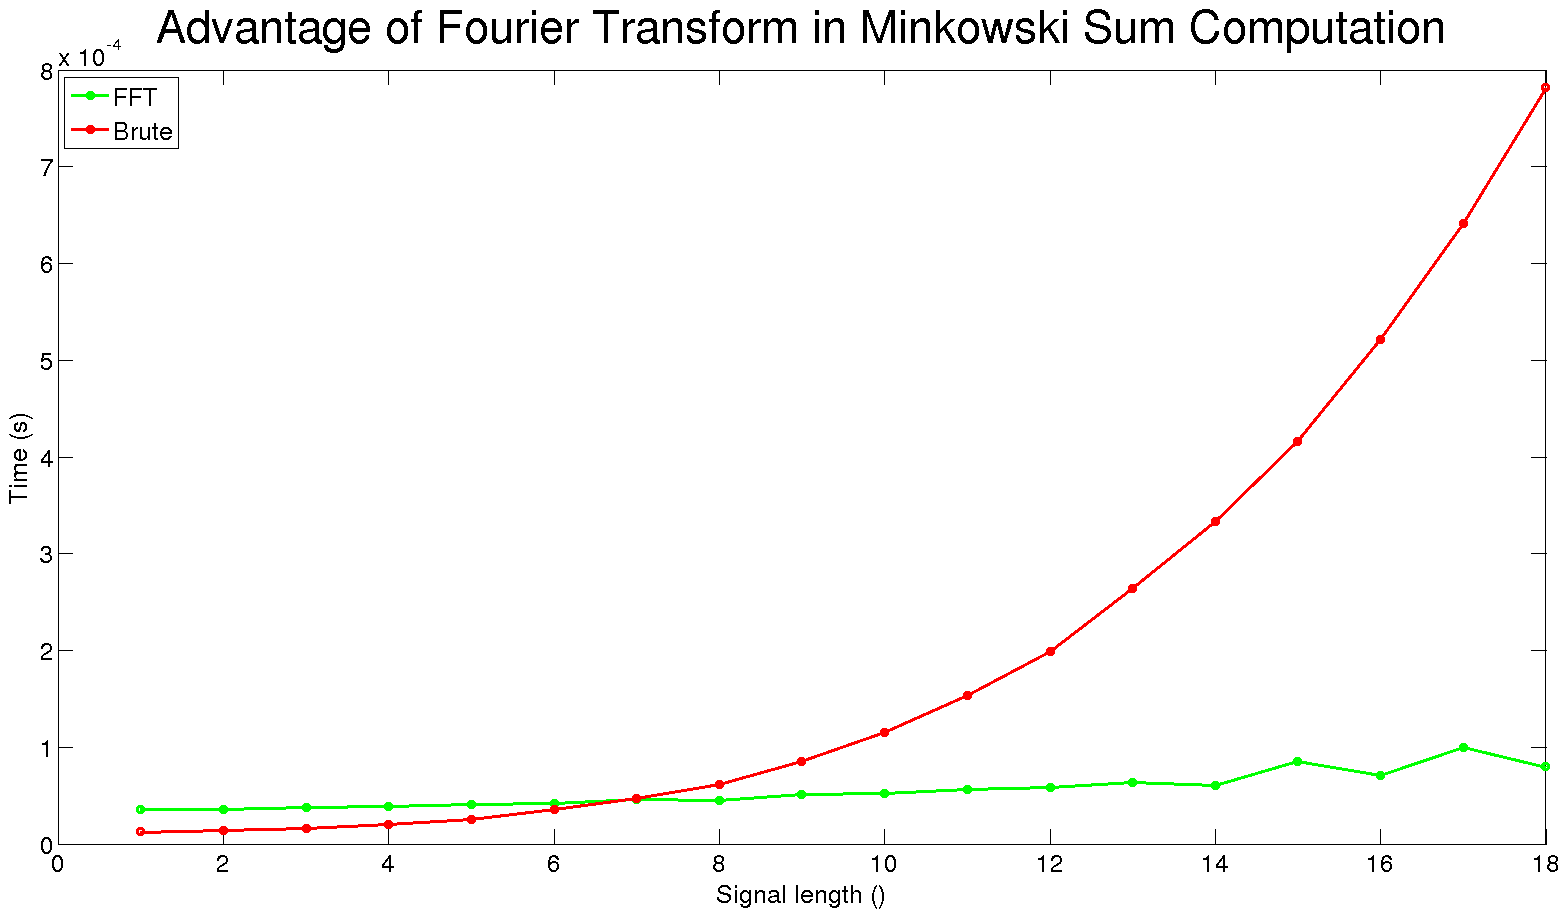
\includegraphics[width=1.0\linewidth]{Figures/fft.png}
  \caption{The comparison of traditional $O(n^2)$ and the FFT $O(nlog(n))$ methods for Minkowski sum
  computations}
  \label{fig:fft}
\end{figure}

\subsection{Spherical vs. Uniform Sampling}

The second major theme of this paper is the signifance of spherical representation in the computation
of Fourier shape descriptors. The main result is based on the efficiency of the implementation of the Minkowski sum of the ball function
$B_0$ with the ball centers $P$. The challenge with uniform sampling is that every voxel in the space
has to check whether it is in the given shape or not to compute the cartesian space signal, an efficiency
challenge even before the FFT computation is done. On the other hand, given the ball centers, the
descriptor computation is as simple as a element-wise product $O(n)$ in the frequency domain.

Figure \ref{fig:spherical} demonstrates the comparison of uniform and spherical representation
in the computation time of Fourier shape descriptors. The input data was randomly generated by two-dimensional
balls and for each number of balls, 100 trials were conducted. Clearly, the spherical approach 
is faster and the main reason it says almost constant is that the element-wise product is
limited to only a handful spheres (at most 10). The results show a preliminary confirmation
of \cite{behandish2016analytic} who have demonstrated similar results with considerably larger
dataset.

\begin{figure}[ht!] 
  \centering
  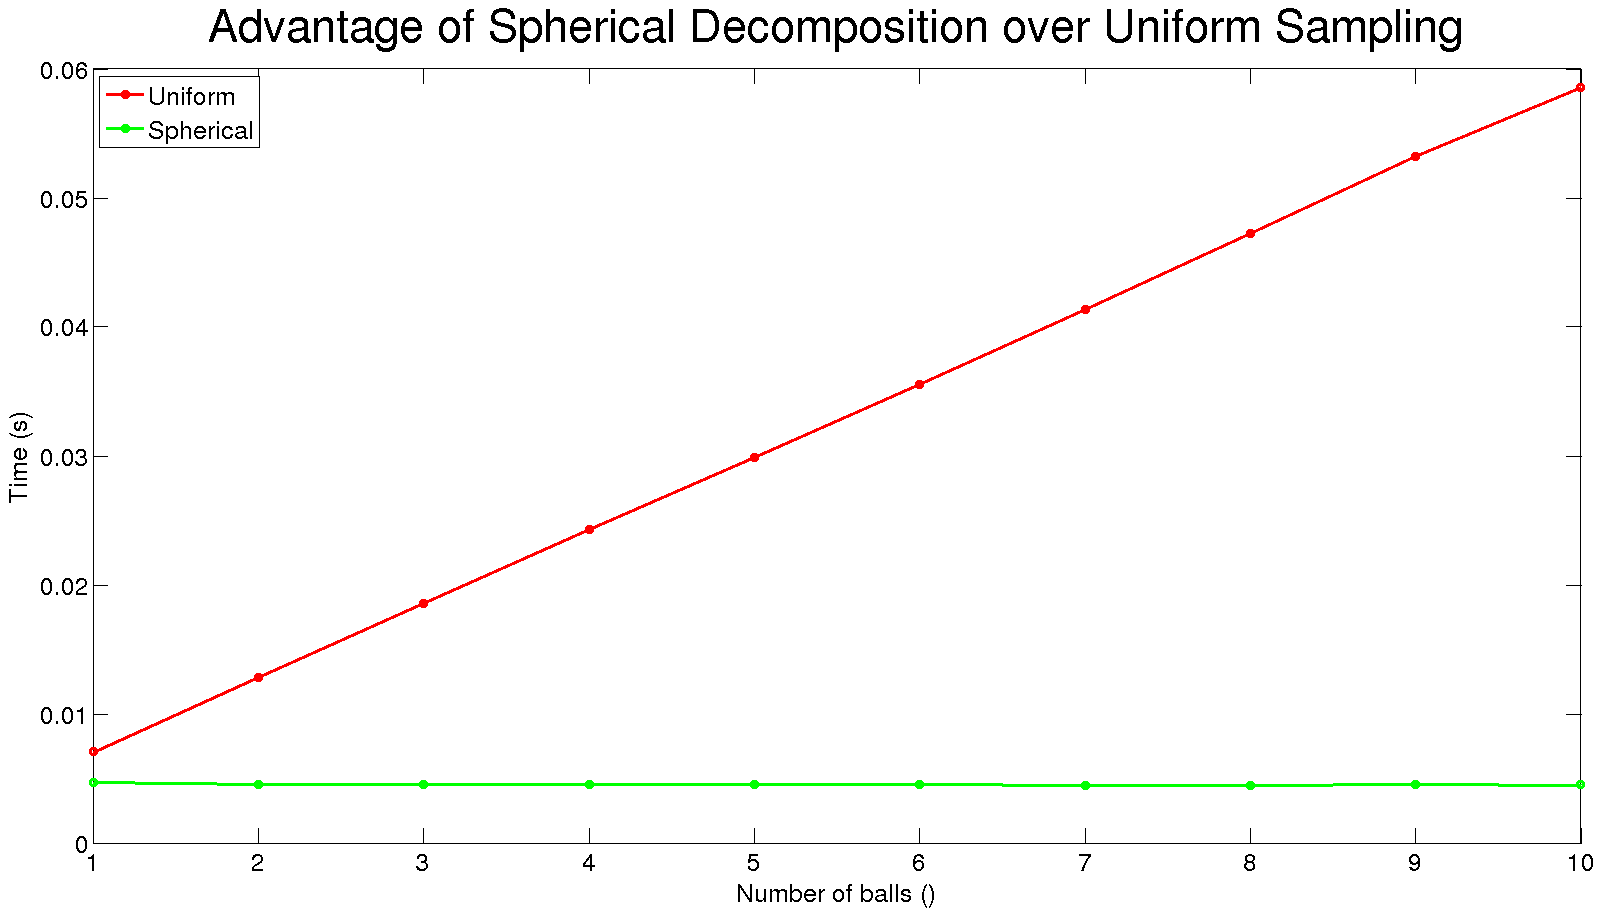
\includegraphics[width=1.0\linewidth]{Figures/spherical.png}
  \caption{The comparison of computation time of Fourier shape descriptors with uniform and spherical representations}
  \label{fig:spherical}
\end{figure}

% -------------------------------------------------------------------------------------------------
% -------------------------------------------------------------------------------------------------
\section{Future Work}

A large number of efficiency improvements can be done to the current framework including but not limited to:

\begin{itemize}
 \item Prioritize frequencies in early-miss tests: \cite{lysenko2013fourier} demonstrates an
 inequality check method which ensures that if a sufficient number of high-frequency values in the
 frequency representation of the intersection shape descriptor is zero, then the conversion can
 be stopped. This would be equivalent to, conceptually, hierarchical planning where first higher-order
 terms are checked. 
 
 \item NFFTs: In the current implementation, to transform the centers of the balls to the frequency 
 domain, a uniform sample over a grid is performed and the ball centers are confined to these values.
 The drawback is that not only the space of shapes are limited but also, unnecessary samples are being
 used in the FFT.
\end{itemize}

In terms of implementation, we would also like to:
\begin{itemize}
 \item Rotations: Incorporation of rotations is vital to any realistic application to robotics.
 However, the interpolation schemes listed in \cite{lysenko2013fourier, kavraki1995computation} are
 not trivial and as far as we know, there are no theoretical convergence proofs.
 \item Higher orders: The current results (along with Lysenko's) are only in 2D, and even our
 motivation paper \cite{behandish2016analytic} only reports results in 3D. The goal would be to 
 replicate results in the configuration space of a robotic arm, 6-7 dimensions at least.
\end{itemize}

% -------------------------------------------------------------------------------------------------
% -------------------------------------------------------------------------------------------------
\section{Conclusion}

In this report, we have presented a number of techniques related to the collision detection, namely
Minkowski sums, spherical decompositions and Fourier transforms. The main motivation of the work
is to observe that collision detection, generically analyzed in cartesian spaces, can also be 
discussed in frequency spaces, and we have studied two recent papers, Lysenko's 2013 paper \cite{lysenko2013fourier}
and Behandish's 2016 paper \cite{behandish2016analytic}. We analyze the main advantages that
underlie these papers, namely the power of FFTs in computing Minkowski sums, and the advantage of 
spherical decompositions over uniform samples (along with NFFTs), and provide preliminary
results from our own implementations that confirm the findings of the authors. Finally, we 
propose methods to combine the strengths of both papers and define the future outlook of this
line of work.

% -------------------------------------------------------------------------------------------------
% -------------------------------------------------------------------------------------------------
\bibliographystyle{unsrt}
\bibliography{minkowski}

\end{document}
